%% ****** Start of file template.aps ****** %
%%
%%
%%   This file is part of the APS files in the REVTeX 4 distribution.
%%   Version 4.0 of REVTeX, August 2001
%%
%%
%%   Copyright (c) 2001 The American Physical Society.
%%
%%   See the REVTeX 4 README file for restrictions and more information.
%%
%
% This is a template for producing manuscripts for use with REVTEX 4.0
% Copy this file to another name and then work on that file.
% That way, you always have this original template file to use.
%
% Group addresses by affiliation; use superscriptaddress for long
% author lists, or if there are many overlapping affiliations.
% For Phys. Rev. appearance, change preprint to twocolumn.
% Choose pra, prb, prc, prd, pre, prl, prstab, or rmp for journal
%  Add 'draft' option to mark overfull boxes with black boxes
%  Add 'showpacs' option to make PACS codes appear
%  Add 'showkeys' option to make keywords appear
\documentclass{revtex4}
%\documentclass[aps,prl,preprint,superscriptaddress]{revtex4}
%\documentclass[aps,prl,twocolumn,groupedaddress]{revtex4}
\usepackage[dvipdf]{graphicx}
%\usepackage{dcolumn}

% You should use BibTeX and apsrev.bst for references
% Choosing a journal automatically selects the correct APS
% BibTeX style file (bst file), so only uncomment the line
% below if necessary.
%\bibliographystyle{apsrev}

\begin{document}

% Use the \preprint command to place your local institutional report
% number in the upper righthand corner of the title page in preprint mode.
% Multiple \preprint commands are allowed.
% Use the 'preprintnumbers' class option to override journal defaults
% to display numbers if necessary
%\preprint{}

%Title of paper
\title{Measurement of Planck's Constant with Light-Emitting Diodes}

% repeat the \author .. \affiliation  etc. as needed
% \email, \thanks, \homepage, \altaffiliation all apply to the current
% author. Explanatory text should go in the []'s, actual e-mail
% address or url should go in the {}'s for \email and \homepage.
% Please use the appropriate macro foreach each type of information

% \affiliation command applies to all authors since the last
% \affiliation command. The \affiliation command should follow the
% other information
% \affiliation can be followed by \email, \homepage, \thanks as well.
\author{Physics 2501: Mechanics and Electromagnetism Laboratory}
%\homepage[]{Your web page}
%\thanks{}
%\altaffiliation{}
\affiliation{Dept. of Physics, University of Connecticut}
%\author{R.T. Jones}
%\affiliation{University of Connecticut}

%Collaboration name if desired (requires use of superscriptaddress
%option in \documentclass). \noaffiliation is required (may also be
%used with the \author command).
%\collaboration can be followed by \email, \homepage, \thanks as well.
%\collaboration{}
%\noaffiliation

\date{\today}

%\begin{abstract}
% insert abstract here
%\end{abstract}

% insert suggested PACS numbers in braces on next line
%\pacs{}
% insert suggested keywords - APS authors don't need to do this
%\keywords{}

%\setlength{\topmargin}{0in}

%\maketitle must follow title, authors, abstract, \pacs, and \keywords
\maketitle

% body of paper here - Use proper section commands
% References should be done using the \cite, \ref, and \label commands

%% The normal text is displayed in two-column format, but special
%% sections spanning both columns can be inserted within the page
%% format so that long equations can be displayed. Use
%% sparingly.
%%\begin{widetext}
%% put long equation here
%%\end{widetext}
%
%% figures should be put into the text as floats.
%% Use the graphics or graphicx packages (distributed with LaTeX2e)
%% and the \includegraphics macro defined in those packages.
%% See the LaTeX Graphics Companion by Michel Goosens, Sebastian Rahtz,
%% and Frank Mittelbach for instance.
%%
%% Here is an example of the general form of a figure:
%% Fill in the caption in the braces of the \caption{} command. Put the label
%% that you will use with \ref{} command in the braces of the \label{} command.
%% Use the figure* environment if the figure should span across the
%% entire page. There is no need to do explicit centering.
%
%%\begin{turnpage}
%% Surround figure environment with turnpage environment for landscape
%% figure
%% \begin{turnpage}
%% \begin{figure}
%% \includegraphics{}%
%% \caption{\label{}}
%% \end{figure}
%% \end{turnpage}
%
%% tables should appear as floats within the text
%%
%% Here is an example of the general form of a table:
%% Fill in the caption in the braces of the \caption{} command. Put the label
%% that you will use with \ref{} command in the braces of the \label{} command.
%% Insert the column specifiers (l, r, c, d, etc.) in the empty braces of the
%% \begin{tabular}{} command.
%% The ruledtabular enviroment adds doubled rules to table and sets a
%% reasonable default table settings.
%% Use the table* environment to get a full-width table in two-column
%% Add \usepackage{longtable} and the longtable (or longtable*}
%% environment for nicely formatted long tables. Or use the the [H]
%% placement option to break a long table (with less control than 
%% in longtable).
%
%
%% Surround table environment with turnpage environment for landscape
%% table
%% \begin{turnpage}
%% \begin{table}
%% \caption{\label{}}
%% \begin{ruledtabular}
%% \begin{tabular}{}
%% \end{tabular}
%% \end{ruledtabular}
%% \end{table}
%% \end{turnpage}
%
%% Specify following sections are appendices. Use \appendix* if there
%% only one appendix.
%%\appendix
%%\section{}
%

\section{Introduction}

Max Planck (1858-1947) was an early pioneer in the field of quantum physics.
Around 1900 Planck developed the concept of energy quantization to explain the
spectral distribution of blackbody radiation~\cite{Planck01}. This idea is
fundamental to the quantum theory of modern physics.  Planck received a Nobel
Prize for his work in the early development of quantum mechanics in 1918.
Interestingly, Planck himself remained skeptical of practical applications
of quantum theory for many years after the implications of proposal were
recognized.

Planck proposed that atoms absorb and emit radiation in discrete
quantities of energy given by
\begin{equation}
\Delta E = nhf
\label{eq:nhf}
\end{equation}
where $f$ is the frequency of vibration of the atom and $n$ is an integer
multiplier.  The factor $h$ in Eq.~\ref{eq:nhf}, which was introduced by
Planck as a proportionality constant between the atomic frequency and the
minimum energy that could be emitted or absorbed by the atom, is known
today as {\em Planck's constant}.  Planck's constant is one of only three
fundamental dimensionful constants in all of Modern Physics, the other two
being the speed of light in vacuum $c$, an Newton's universal gravitational
constant $G$.  Planck conceived of $h$ as measuring the smallest discrete
amount of energy that an atom can radiate or absorb, thus decreasing or
increasing its internal energy by the amount $\Delta E$.  The key element
of Planck's hypothesis, on which its success in explaining the blackbody
radiation spectrum depended, is that the minimum energy quantum be
proportional to the frequency of the radiation emitted.  Therefore the
fundamental constant does not have units of energy, but energy divided
by frequency, or energy times time.

The integer $n$ in Eq.~\ref{eq:nhf} allows for the case where the
emission or absorption occurs in multiple steps at once, like someone
climbing or descending stairs several steps at a time.  He included the
possibility that $n>1$ because there was nothing in the success of his
blackbody spectrum calculation that required the steps to happen one at
a time.  Later in 1905, Albert Einstein (1879-1955) published a
paper~\cite{Einstein05} in which he used Planck's energy quantization
principle to explain the photoelectric effect. The photoelectric effect
is in many ways the reverse of what occurs in a light-emitting diode when
a current passes through it and produces light.  In the photoelectric effect,
light from an external source shining on an electrode in a circuit causes
current to flow through the circuit.  The current is the result of electrons
being liberated from the surface of the electrode where they are ordinarily
bound to atoms, so that they are free to flow through the circuit, as a
consequence of the radiant energy of the light being absorbed by atoms in
the electrode surface.  Einstein asserted that the electrons absorbed one
quantum of electromagnetic energy at a time, and that the energy of this
quantum (photon) is
\begin{equation}
E = hf = \frac{hc}{\lambda}
\label{eq:hf}
\end{equation}
where $c$ is the speed of light in vacuum, and $\lambda$ is the wavelength
of the light incident on the electrode.  Einstein argued that an electron
would only be ejected if the frequency of the light (and hence the energy
of the photon) was greater than the energy binding the electron to the metal.
Einstein received the Nobel Prize in Physics for this work in 1921.  This is
essentially the same idea as Planck's, except that Einstein restricted the
allowed values of $n$ to 1.

Niels Bohr (1885-1962) used Planck's ideas on
the quantization of energy as a starting point in developing the modern
theory for the hydrogen atom.  Robert Millikan made the first measurement
of Planck's constant in 1912~\cite{Millikan12}.
The best current value for Planck's constant
is $h = 6.6260689633\times 10^{-34}$~J~s =
$4.136054727\times 10^{-15}$~eV~s~\cite{PDG2010}.

In this experiment, you will use the current-voltage relationship of a set of
light-emitting diodes (LEDs) to measure Planck's constant. An LED is a
semiconductor device that emits electromagnetic radiation at optical and
infrared frequencies when an electric current passes through it. The device
consists of a semiconductor material, such as GaAs, GaP, or SiC, into which
small impurities of different kinds have been introduced.

A semiconductor is a material whose response to electrical potential is
in some ways like a conductor and in some ways like an insulator.  When an
electric potential is placed across a sample of pure semiconductor crystal
at room temperature, it behaves like an insulator and no current flows
through it.  However, if impurities are present in the semiconductor crystal,
even in microscopic amounts, these impurities introduce free charges to the 
semiconductor crystal lattice, and it conducts current in the direction of
the applied electric field.  The substitution of impurity atoms for those
of the original semiconductor crystal modifies it in one of two basic ways:
either the impurity atom has more valence electrons than the atom that would
normally be found at a given crystal site, or it has less.  If it has more,
the extra valence electrons detach themselves from their impurity atoms and
are free to move about the crystal.  Adding impurities of this type to a
semiconductor is called {\em $n-type$ doping} because the free charges are
electrons and carry negative charge.  However, if the impurity atom has
fewer electrons than the atom that would normally be found at its site then it
acts like a ``hole'' in the regular electron distribution across the crystal.
This hole is free to move in the sense that nearby electrons can move into
it, eliminating the old hole but leaving behind a new one at the site from
which the electron came.  Adding impurities of this type to a semiconductor
is called {\em $p-type$ doping} because the mass motion of all of the
electrons a crystal of this type behaves as if there were just a few
positive charges (i.e. holes) that are free to move about the crystal.

An LED is constructed starting with a single piece of pure semiconductor,
and doping one half of it with $n-type$ impurities and the other half with
$p-type$.  Where the two dopings meet is called a {\em junction}.  All of
the interest the the behavior of a semiconductor device is focused on what
takes place at this junction between p-type and n-type material. Because
they are always in motion, the free electrons on the n-side of the junction
sometimes wander over onto the p-side and ``annihilate'' some of the holes
that are plentiful there by falling into them.  Likewise a hole from the
p-side sometimes wanders over onto the n-side and ``eats'' a free electron
there, so the both disappear.  The result is that the region of the junction
gets depleted of free charges, so that current that flows freely in the
interior of either the p-side or n-side does not conduct across the junction.
This situation is represented in the first panel of Fig.~\ref{junctionfig}.
The fact that some electrons and some holes have gotten trapped on the
``wrong'' side of the junction means that the there is an overall positive
charge left behind on the n-side and an overall negative charge on the p-side
of the junction, leading to a spontaneous electric field in the vicinity of
the junction.  This spontaneous electric field at the junction is a natural
consequence of the mobility of charges in doped semiconductor; it is not
produced by an external voltage source, nor can it be used to do real work,
such as drive current in an external circuit.  It is part of the static
equilibrium of the charges in the region of the junction, which prevents
all of the free electrons from the n-side from eventually wandering over
to the p-side and disappearing into a hole, and vice versa, and it exists
only in a thin layer (normally a few microns thick) around the junction.

\begin{figure}
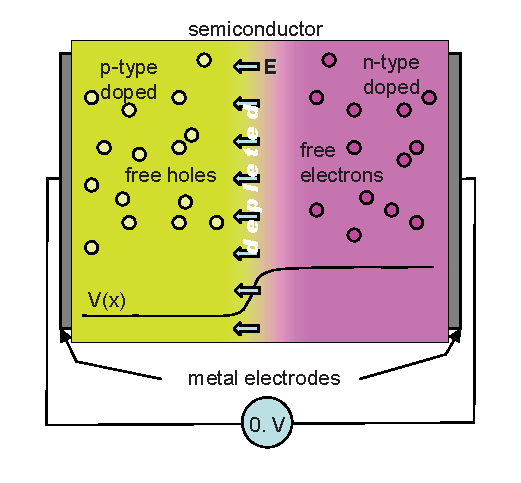
\includegraphics[width=2.6in]{junctionfiga.eps}
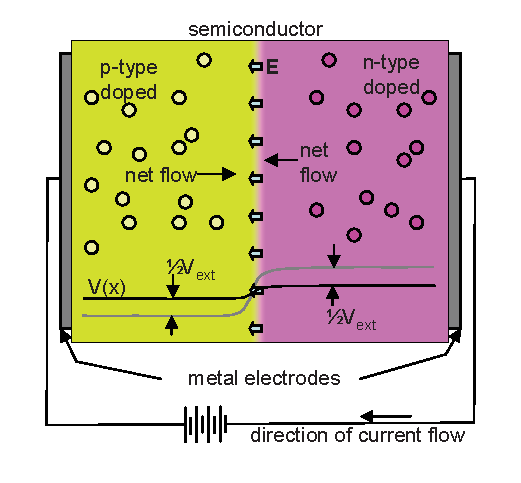
\includegraphics[width=2.6in]{junctionfigb.eps}
\caption{\label{junctionfig}
Behavioral diagram of a bipolar semiconductor diode shown in its unbiased
state (left panel) and in its forward-biased state (right panel).  The
curve labeled $V(x)$ in both figures represents the background potential
in which the free charge carriers move.  The arrows at the junction
represent the electric field, which is the negative gradient of the potential.
Note in the second panel that even in the forward-biased state there is still
a residual potential barrier at the junction, which the charge carriers are
able to overcome by their thermal (kinetic) energy.  The unbiased $V(x)$
function is shown by the grayed out curve in the right-hand panel for 
comparison.}
\end{figure}

The spontaneous electric field at the junction can be approximated by a
uniform field like the one that exists between the plates of a parallel plate
capacitor.  Using Gauss' Law, one can compute the potential difference
between the bulk media on the n-side and p-side of the junction.  The
potential is illustrated by the blue curve in Fig.~\ref{junctionfig}a.  The
exact value of this junction potential difference $V_j$ depends on the type
of semiconductor and the doping materials, but is typically on the order of
a volt.  This potential can be overcome by imposing an external potential
difference on the two sides of the junction, effectively opposing the
spontaneous field and driving free electrons and holes back into the
depleted region at the junction.  If the external potential $V_{ext}$ is raised
all the way to $V_j$ then the barrier is completely removed and the junction
behaves like a conductor, albeit a fairly poor one because only the valence
electrons/holes of the impurity sites are free to move.

If an experiment measuring the current through the junction as a function
of the external voltage $V_{ext}$ were conducted at absolute zero temperature
then no current would flow until the external potential reaches $V_j$.
However, at finite temperature the charges have enough thermal energy to
sometimes jump over the barrier, the probability of which is greatly increased
by using $V_{ext}$ to lowering the junction potential, as illustrated in
Fig.~\ref{junctionfig}b.  A very general principle from statistical mechanics
states that if a system is in equilibrium at temperature $T$ then the
probability that it will be detected at an excited level with an energy
$\Delta E$ above the ground state is given by the so-called {\em
Boltzmann factor}
\begin{equation}
{\cal P} \propto e^{-\frac{\Delta E}{nk_{_B} T}}
\label{eq:Boltz}
\end{equation}
where $T$ is the absolute temperature of the semiconductor in Kelvin
and $k_{_B}$ is Boltzmann's constant.  The {\em ideality factor} $n$
is a dimensionless number that varies from 1 to 2, and sometimes higher,
depending on the fabrication process and semiconductor material.  The
LED's used in this experiment typically have ideality factors in the
range 1.5-2.0 for current levels of interest in this measurement.

In the situation illustrated in Fig.~\ref{junctionfig},
$\Delta E = e(V_j-V_{ext})$ where $e$ is the absolute value of the charge
of an electron.  Interpreting the current across the junction
as proportional to the probability ${\cal P}$ in Eq.~\ref{eq:Boltz}, this
leads to the following prediction for how the current $I$ depends on $V_{ext}$.
\begin{equation}
I \propto e^{\frac{eV_{ext}-eV_j}{nk_{_B} T}}
\label{eq:VI1}
\end{equation}
A semiconductor device whose current-voltage relationship are described
by Eq.~\ref{eq:VI1} is known as a {\em diode}.  Note that setting $V_{ext}$
to a negative value (reverse bias) only drives the device further into
cutoff, while a positive value $V_{ext}$ above a certain minimum value
(forward bias) can cause current to flow.  In this sense, a diode is like
a one-way valve for electric current.

In order to understand how current flows through a pn diode it
is important to remember that holes are still the principal charge carriers
on the p-side, while electrons are responsible for the current on the n-side.
A useful picture of a forward-biased diode is the electrons flow into the
junction region from the n-side, holes flow into the junction from the p-side,
and the two combine and disappear at the junction.  This useful picture for
understanding how a light-emitting diode works is illustrated in
Fig~\ref{junctionfig}.  Every time an electron
flowing into the junction region from the n-side combines with a hole flowing
into the junction region from the p-side, an energy approximately equal to
$eV_j$ is released.  This release of energy takes a variety of forms, one
of which is the emission of light.  Einstein's equation Eq.~\ref{eq:hf}
provides a relationship between the junction voltage and the wavelength of
the light that will be emitted.
\begin{equation}
eV_j = \frac{hc}{\lambda}
\label{eq:Vjlambda}
\end{equation}
If the junction is buried inside the bulk semiconductor then these photons
are reabsorbed and converted into heat inside the diode, but if the diode is
engineered to place the junction near the surface then a large fraction of
the light can escape.  This specially engineered device is called a
light-emitting diode.

To make contact with Planck's constant, it is necessary to compare the
current-voltage curves of several different light-emitting diodes with
different $V_j$ values.  A device with $V_j$ near 1.9~V produces red light,
while one with $V_j$ up around 3.0~V emits blue light.  In this experiment
you will measure the V-I curves of several LEDs, varying in color from red
to blue.  Manufacturers of LED devices specify what wavelength of the light
they emit.  This provides you with the values of $\lambda$ to be substituted
into Eq.~\ref{eq:Vjlambda}.  To determine the corresponding values for $V_j$
you will the following procedure.  Fitting the measured V-I curves for the
different LEDs to Eq.~\ref{eq:VI1}, you will determine the value of $V_{ext}$
for each diode that corresponds to a standard current value $I_0$.  A value
like 10~$\mu$A for $I_0$ would be a good choice.  Now you have a value of
$V_{ext}$ for the red diode, a different value for the yellow diode, and so
on.  It follows from Eq.~\ref{eq:VI1} that
\begin{equation}
V_{ext} = V_j + C
\label{eq:linfit}
\end{equation}
where all of the factors $n$, $k_{_B} T$, $\log I_0$, and the electron charge
$e$ have been lumped together with the unknown proportionality constant from
Eq.~\ref{eq:VI1} and designated by the unknown constant $C$.  The beauty
of this method is that you do not need to know the value of $C$ in order
to extract a value for $h$ from your data.  Eq.~\ref{eq:hf} states
that $eV_j$ is proportional to $c/\lambda$ with proportionality constant
$h$.  It follows that, no matter what the exact value of $C$ might be,
$eV_{ext}$ is a linear function of $c/\lambda$ with slope $h$.  To extract
a value of $h$ from the values of $V_{ext}$ at standard current $I_0$
that you measured for each diode, you will plot $V_{ext}$ versus
$c/\lambda$ and fit your data to a straight line.  The fit will provide you
with a best-fit value for the slope, and also its error.  Multiplying these
two numbers by the electron charge $e$ gives your measured value for $h$
and its measurement uncertainty, or error.

%\begin{table}
%\caption{\label{displacementfig}
%Nkmg cktetchv cpf dtkfigu, cpf vq uocnngt uvtwevwtgu
%nkmgcvqou cpf pwengk, vjku ukorng oqfgn ikxgu korqtvcpv kpukijv kpvq
%vjgdgjcxkqt qh gxgp vjg oquv eqornkecvgf uauvgou yjgp vjgkt fapcokeu
%ctgiqxgtpgf da uocnn fgrctvwtgu htqo gswknkdtkwo.}
%\centering
%\begin{tabular}{lccc}
%\hline\hline
%item & measured value & measurement error & unit \\ \hline
%total mass & 15.67 & 0.02 & kg \\
%length eyes-tailfin & 14.6 & 0.05 & cm \\
%height belly-dorsal & 3.98 & 0.05 & cm \\
%flash response time & 1.23 & 0.15 & s \\
%total turn time & 1.08 & 0.05 & s \\
%turn radius & 0.72 & 0.15 & cm \\
%maximum turn velocity & 22.1 & 0.5 & m/s \\
%\hline\hline
%\end{tabular}
%\end{table}

\section{Method}

\begin{figure}
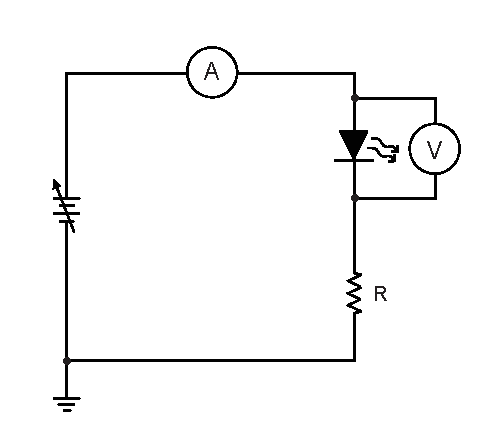
\includegraphics[width=2in]{VIcircuit.eps}
\caption{\label{VIcircuit}
Diagram of the circuit used to measure V-I curves for the LEDs examined
in this experiment.  The resistor $R$ is present to protect the LED against
accidental over-voltage.  Its value should be no less than 100~$\Omega$.}
\end{figure}

The main component of the apparatus is a circuit board containing 6 LEDs,
each with a different emission wavelength. A particular LED should be connected
to the circuit shown in Fig.~\ref{VIcircuit}, and the current and voltage 
measured as the external voltage from the power supply is varied. Connect
the power supply and ammeter to the + (red) and - (black) terminals on the
LED board so that the current-limiting resistor is included in the circuit.
Be sure the power supply is off and the voltage knob is set to zero before
you modify the circuit.  Check that the voltmeter measures the voltage
directly across the LED only, i.e. not including the resistor. Turn the power
supply on and {\em very slowly} increases the voltage until the LED just
starts to glow. Continually monitor the current so that you do not exceed
the maximum current of 20~mA. Measure the current as a function of the
voltage measured on the voltmeter.  Make sure that your measurements extend
all the way down to where you observe the minimum detectable current on the
ammeter, and up at least as high as the point where the glow of the LED
becomes visible.

Repeat these measurements of the V-I curves for each of the other diodes,
noting that 5 of them have a maximum current rating of 20~mA.  The infrared
LED has a 100~mA rating.

Plot graphs of current (ordinate) vs voltage (abscissa) for each LED. The
experimental problem here is how to determine $I_0$, the reference current
to be used in the comparison between the various LEDs.  If you use a semi-log
plot to view the V-I curves (set the current axis to use a log scale), each
of the curves should appear as an S-curve.  At the low end of the curves you
should see a bending of the curve toward lower slope.  This is caused by 
leakage currents in the circuit that are not flowing through the diode
junction, such as the small current that flows through the voltmeter.
A similar bend to lower slope is also seen at the high-current end of the
curve.  Reasons for the bending at the high-current end are that above a 
few mA current the ideality factor of the diode begins to grow, and the
resistance of the bulk doped material in the diode begins to play a role.
Above the point where the current begins to rise with voltage and before
the current reaches 1~mA there should be a clear range of exponential
behavior (linear on a semi-log plot).  Chose a common value for $I_0$
that is inside this safe range for all of the diodes.

Based on visual inspection of your V-I curves on a semi-log graph, chose
the range of clean exponential behavior for each of your LEDs and fit the
data within that range to an exponential.  The simplest way to do this is
to compute $x=\log(I/I_0)$ for each data point, and then fit a straight line
to $V_{ext}$ versus $x$.  Only include points in the fit that lie within the
range determined above.  It is a valid procedure to exclude from the fit
data points from the beginning and the end of your scan, but do not exclude
individual points within the accepted range, as this would bias your result.
The y-intercept of the best-fit line is the value of $V_0$
for this LED, to be used in the next step.  Make sure that you use your
measurement uncertainty $\Delta V_{ext}$ on the values of $V_{ext}$ when
you compute the $\chi^2$ that you minimize in the fit.  The slope of these
best-fit lines is given by the factor $nk_{_B}T/e$.  Determine $n$ for each
of the diodes, verifying that it is within the range 1.5-2.0 or nearby.
If this is not the case for one of your diodes, it is evidence that you
have made a poor choice for the linear region, and should go back and
survey the $V-I$ curve again and find a more appropriate fit range.

By the above procedure, you should now have six values of $V_0$ and their
corresponding errors, one set for each of the six LEDs.  Record the emission
wavelengths of each of the LEDs and convert them to frequency through the
relation $f=c/\lambda$.  Now make a graph of $V_0$ versus $f$ for the six
LEDs.  Add error bars showing the errors on $V_0$.  Do a linear fit to these
data.  The best-fit slope is your value for $h/e$, which is the numerical
value of Planck's constant in units of eV~s.  Use the jack-knife procedure
to estimate the error on the best-fit slope, and report this as the error
on your measured value of $h$.

If you did a careful job with the $V-I$ curve measurements, you should
find that the $\chi^2$ value of the fit of $V_0$ versus $f$ is very large,
indicating a poor fit.  Thus you may find a value for $h/e$ that has a 
very small error, compared to what you would guess visually is the uncertainty
in the slope just by looking at the plot.  This discrepancy comes about
because the proportionality factor in Eq.~\ref{eq:Boltz} can be different
for each diode, whereas the model assumes that they are all the same.
A simple way to incorporate this systematic error into your analysis is
to add a uniform constant to the measurement errors on the $V_0$ values and
increase the additive constant until the $\chi^2$ of the overall fit comes
into the range expected for an acceptable fit.  This will not change the
measured value for $h/e$ by an appreciable amount, but the error on the
measured value will increase to a point where a comparison with the
accepted value becomes realistically possible.


\begin{acknowledgments}
This document was updated by Prof. Richard Jones, based on an original
write-up by Prof. Doug Hamilton (2004).
\end{acknowledgments}

%% Create the reference section using BibTeX:
%\bibliography{revtex4}

\begin{thebibliography}{9}

\bibitem{Planck01}
M. Planck, {\em Uber das Gesetz der Energieverteilung im Normalspektrum},
Ann.\ d.\ Physik {\bf 4} (1901) p. 553.
\bibitem{Einstein05}
A. Einstein, {\em Uber einen die Erzeugung und Verwandlung des Lichtes
betreffenden heuristischen Gesichtspunkt}, Ann.\ d.\ Physik {\bf 17} (1905)
p. 132.
\bibitem{Millikan12}
R.A.~Millikan, {\em A Direct Photoelectric Determination of Planck's ``h''},
Phys.\ Rev.\ {\bf 7} (1916) p. 355.
\bibitem{PDG2010}
Particle Data Group, {\em Review of Particle Physics}, Jour.\ Phys.\ G
{\bf 37}, no. 7A (2010) p. 1.
\end{thebibliography}

\end{document}
%%
%% ****** End of file template.aps ******
%
%
